% Vietnamese translation for OI Public Library
% Source-PDF: IOI中国国家候选队论文/2000/张辰论文.pdf
\documentclass[11pt]{article}
\usepackage{oipl-vn}
\usepackage{tikz}
\usetikzlibrary{arrows.meta}

\title{Đặc điểm và ứng dụng của quy hoạch động}
\author{Zhang Chen}
\date{}

\begin{document}
\maketitle

\origtitle{Characteristics and applications of dynamic programming}
\sourcepath{IOI China candidate team papers / 2000 / Zhang Chen.pdf}

\paragraph{Từ khóa.}
Quy hoạch động; giai đoạn.

\section*{Tóm tắt}

Quy hoạch động là một thuật toán thường gặp trong thi tin học. Nội dung chính
của bài viết này là phân tích các đặc điểm của nó.

Phần đầu của bài viết trước hết khảo sát bản chất của quy hoạch động, vì các
đặc điểm của quy hoạch động do chính bản chất ấy quyết định. Phần thứ hai
phân tích ba đặc điểm: tính đa dạng, tính khuôn mẫu và tính kỹ thuật của quy
hoạch động, từ hai góc độ thiết kế và cài đặt. Phần thứ ba so sánh quy hoạch
động với ba thuật toán liên quan: truy hồi, tìm kiếm và luồng mạng, qua đó
tìm hiểu một số đặc điểm sâu hơn của quy hoạch động.

Trong khi phân tích các đặc điểm của quy hoạch động, bài viết cũng dựa vào
những đặc điểm ấy để phân tích khi giải bài ta nên tận dụng chúng như thế
nào, và nên vận dụng quy hoạch động ra sao. Điều này có ý nghĩa định hướng
nhất định đối với thực hành giải bài.

\tableofcontents

\section{Dẫn nhập}

Quy hoạch động là một phương tiện quan trọng trong lập trình giải bài, và
ngày càng được dùng phổ biến trong các kỳ thi tin học hiện nay. Trong vài năm
gần đây, hầu như kỳ thi tin học nào, lớn hay nhỏ, cũng đều kiểm tra nội dung
này. Vì vậy, làm thế nào để hiểu sâu hơn về quy hoạch động, từ đó dùng hiệu
quả hơn vũ khí mạnh mẽ này khi giải bài, là một vấn đề đáng nghiên cứu.

Muốn nắm được kỹ thuật ứng dụng quy hoạch động, ta phải hiểu các đặc điểm ở
nhiều mặt của nó. Trước hết là phải nhìn sâu vào bản chất của quy hoạch động.

\section{Bản chất của quy hoạch động}

Quy hoạch động ra đời vào đầu thập niên 1950 để giải quyết một lớp bài toán
quyết định nhiều giai đoạn. Vậy bài toán như thế nào được gọi là bài toán
quyết định nhiều giai đoạn?

\subsection{Bài toán quyết định nhiều giai đoạn}

Khi nói đến bài toán quyết định nhiều giai đoạn, người ta rất dễ nêu ví dụ
sau.

\paragraph{Ví dụ 1. Bài toán đường đi ngắn nhất trong đồ thị nhiều tầng.}
Hãy tìm đường đi ngắn nhất từ \(A_1\) đến \(D_1\) trong đồ thị dưới đây.

\begin{center}
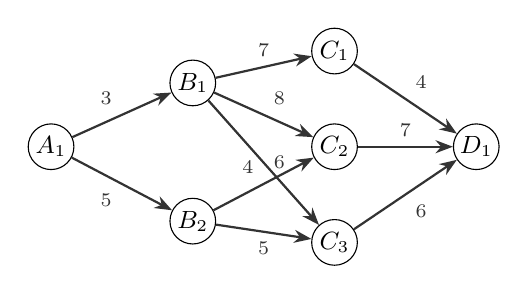
\begin{tikzpicture}[
  v/.style={circle,draw,minimum size=0.58cm,inner sep=0pt,font=\small},
  edge/.style={-{Stealth[length=2.2mm]},black!80,thick},
  every node/.style={font=\scriptsize},
  x=0.9cm,y=0.9cm
]
  \node[v] (a) at (0,0) {$A_1$};
  \node[v] (b1) at (2,0.9) {$B_1$};
  \node[v] (b2) at (2,-1.05) {$B_2$};
  \node[v] (c1) at (4,1.35) {$C_1$};
  \node[v] (c2) at (4,0) {$C_2$};
  \node[v] (c3) at (4,-1.35) {$C_3$};
  \node[v] (d) at (6,0) {$D_1$};

  \draw[edge] (a)--node[above left]{3}(b1);
  \draw[edge] (a)--node[below left]{5}(b2);
  \draw[edge] (b1)--node[above]{7}(c1);
  \draw[edge] (b1)--node[above right]{8}(c2);
  \draw[edge] (b1)--node[right]{6}(c3);
  \draw[edge] (b2)--node[above left]{4}(c2);
  \draw[edge] (b2)--node[below]{5}(c3);
  \draw[edge] (c1)--node[above right]{4}(d);
  \draw[edge] (c2)--node[above]{7}(d);
  \draw[edge] (c3)--node[below right]{6}(d);
\end{tikzpicture}
\end{center}

Trong đồ thị này, các cạnh chỉ đi từ một tầng sang tầng kế tiếp:
\[
\begin{array}{c}
A_1\to B_1\ (3),\quad A_1\to B_2\ (5),\\
B_1\to C_1\ (7),\quad B_1\to C_2\ (8),\quad B_1\to C_3\ (6),\\
B_2\to C_2\ (4),\quad B_2\to C_3\ (5),\\
C_1\to D_1\ (4),\quad C_2\to D_1\ (7),\quad C_3\to D_1\ (6).
\end{array}
\]

Quan sát kỹ đồ thị này, ta thấy nó có một đặc điểm. Nếu chia các đỉnh trong
đồ thị thành bốn lớp \(A,B,C,D\), thì mọi cạnh đều nằm giữa hai lớp kề nhau
và đều hướng từ lớp trước sang lớp sau. Như vậy các cạnh trong đồ thị được
chia thành ba loại: \(A\to B\), \(B\to C\), \(C\to D\). Ta cần chọn một cạnh
từ mỗi loại để tạo thành một đường đi từ \(A_1\) đến \(D_1\), và đường đi ấy
phải là ngắn nhất trong tất cả các đường như vậy.

Từ ví dụ trên, ta có thể hiểu đại khái thế nào là bài toán quyết định nhiều
giai đoạn. Định nghĩa chính xác hơn như sau:

\begin{quote}
Quá trình quyết định nhiều giai đoạn là một lớp quá trình hoạt động đặc biệt:
bài toán có thể được phân rã theo thứ tự thời gian thành một số giai đoạn có
liên hệ với nhau; ở mỗi giai đoạn đều phải đưa ra quyết định, và quyết định
của toàn bộ quá trình là một dãy quyết định~\cite{operations}. Bài toán yêu
cầu làm cho hiệu quả tổng thể của cả hoạt động đạt tối ưu được gọi là bài
toán quyết định nhiều giai đoạn.
\end{quote}

Từ định nghĩa trên, ta thấy rõ lớp bài toán này có hai yếu tố: giai đoạn và
quyết định.

\subsection{Giai đoạn và trạng thái}

\term{Giai đoạn}: phân rã quá trình của bài toán đã cho, theo đặc trưng thời
gian hoặc không gian, thành một số giai đoạn có liên hệ với nhau, để lần lượt
tìm lời giải cho từng giai đoạn. Biến giai đoạn thường được ký hiệu là
\(k\)~\cite{operations}.

Giai đoạn là thuộc tính của bài toán. Trong bài toán quyết định nhiều giai
đoạn thường tồn tại một số giai đoạn; ví dụ trên có bốn giai đoạn \(A,B,C,D\).
Trong tình huống thông thường, giai đoạn liên quan đến thời gian; nhưng trong
rất nhiều bài toán, đặc biệt theo cảm nhận của tác giả là trong các bài toán
tin học, giai đoạn không liên quan đến thời gian. Từ định nghĩa giai đoạn, có
thể thấy hai đặc điểm của nó: ``liên hệ với nhau'' và ``có thứ tự''.

Các giai đoạn liên hệ với nhau như thế nào? Thông qua trạng thái và chuyển
trạng thái.

\term{Trạng thái}: điều kiện khách quan ở đầu mỗi giai đoạn được gọi là trạng
thái. Biến mô tả trạng thái của từng giai đoạn được gọi là biến trạng thái;
thường dùng \(s_k\) để chỉ biến trạng thái ở giai đoạn \(k\). Tập các giá trị
của biến trạng thái \(s_k\) được gọi là tập trạng thái, ký hiệu
\(S_k\)~\cite{operations}.

Trạng thái là thuộc tính của giai đoạn. Mỗi giai đoạn thường chứa một số
trạng thái, dùng để mô tả tình huống khách quan khi bài toán phát triển đến
giai đoạn ấy. Trong ví dụ trên, sau khi người đi đường xuất phát từ \(A_1\)
và đi qua hai giai đoạn, có thể xảy ra ba tình huống: đang ở \(C_1\), \(C_2\)
hoặc \(C_3\). Vì vậy giai đoạn thứ ba có ba trạng thái
\(S_3=\{C_1,C_2,C_3\}\).

Trạng thái của mỗi giai đoạn đều do trạng thái của các giai đoạn trước
``biến đổi'' theo một cách nào đó mà thành; sự ``biến đổi'' này gọi là
chuyển trạng thái. Trong ví dụ, đỉnh \(C_3\) có thể đi từ \(B_1\), cũng có
thể đi từ \(B_2\). Việc đi từ trạng thái \(B_1\) hoặc \(B_2\) của giai đoạn 2
đến trạng thái \(C_3\) của giai đoạn 3 chính là chuyển trạng thái. Chuyển
trạng thái là con đường sinh ra trạng thái, cũng là con đường nối các giai
đoạn với nhau.

Đến đây có thể nêu một điều kiện quan trọng để áp dụng quy hoạch động. Sau
khi sắp xếp các giai đoạn theo một thứ tự nhất định, đối với một trạng thái
cho trước của một giai đoạn, trạng thái của các giai đoạn trước không thể
trực tiếp ảnh hưởng đến sự phát triển tương lai của nó, mà chỉ có thể ảnh
hưởng thông qua trạng thái hiện tại này. Nói cách khác, mỗi trạng thái là
``một tóm lược đầy đủ của lịch sử quá khứ''~\cite{operations}. Đây là tính
không hậu hiệu. Tính chất này sẽ còn được giải thích ở phần sau.

\subsection{Quyết định và chiến lược}

Giai đoạn và trạng thái ở trên chỉ là một mặt của bài toán quyết định nhiều
giai đoạn; dưới đây là yếu tố ở mặt kia: quyết định.

\term{Quyết định}: khi trạng thái của các giai đoạn đã được cố định, ta có
thể đưa ra các lựa chọn khác nhau, từ đó xác định trạng thái ở giai đoạn
tiếp theo; lựa chọn ấy gọi là quyết định. Biến biểu diễn quyết định gọi là
biến quyết định, thường dùng \(u_k(s_k)\) để biểu diễn biến quyết định ở giai
đoạn \(k\) khi trạng thái là \(s_k\). Trong bài toán thực tế, giá trị của
biến quyết định thường bị giới hạn trong một phạm vi nhất định; phạm vi này
gọi là tập quyết định cho phép. Thường dùng \(D_k(s_k)\) để biểu diễn tập
quyết định cho phép xuất phát từ trạng thái \(s_k\) ở giai đoạn \(k\). Rõ
ràng \(u_k(s_k)\in D_k(s_k)\)~\cite{operations}.

Quyết định là thuộc tính của lời giải. Mục đích của quyết định là ``xác định
trạng thái ở giai đoạn tiếp theo''. Quay lại ví dụ trên, từ trạng thái \(B_1\)
của giai đoạn 2 có ba con đường, tức ba quyết định, lần lượt dẫn đến ba trạng
thái \(C_1,C_2,C_3\) của giai đoạn 3; do đó
\[
  D_2(B_1)=\{C_1,C_2,C_3\}.
\]

Có quyết định rồi, ta có thể định nghĩa chuyển trạng thái: trong quy hoạch
động, trạng thái ở giai đoạn hiện tại thường là kết quả của trạng thái và
quyết định ở giai đoạn trước. Quá trình dùng trạng thái \(s_k\) của giai
đoạn \(k\) và quyết định \(u_k\) của giai đoạn này để xác định trạng thái
\(s_{k+1}\) của giai đoạn \(k+1\) gọi là chuyển trạng thái. Dạng hình thức
của quy luật chuyển trạng thái,
\[
  s_{k+1}=T_k(s_k,u_k),
\]
được gọi là phương trình chuyển trạng thái.

Nhìn như vậy, dường như quyết định và chuyển trạng thái có một mối liên hệ
nào đó. Theo cách hiểu của tác giả, chuyển trạng thái là mục đích của quyết
định, còn quyết định là con đường để chuyển trạng thái.

Sau khi quyết định ở các giai đoạn được xác định, dãy quyết định của toàn bộ
bài toán tạo thành một \term{chiến lược}, ký hiệu
\[
  p_{1,n}=\{u_1(s_1),u_2(s_2),\ldots,u_n(s_n)\}.
\]
Đối với mỗi bài toán thực tế, các chiến lược có thể chọn nằm trong một phạm
vi nhất định, gọi là tập chiến lược cho phép, ký hiệu \(P_{1,n}\). Chiến lược
làm cho toàn bộ bài toán đạt hiệu quả tốt nhất là chiến lược tối ưu
~\cite{operations}.

Đến đây lại có thể nêu một tiền đề để dùng quy hoạch động: chiến lược tối ưu
của quá trình phải có tính chất sau. Bất kể trạng thái ban đầu và quyết định
ban đầu là gì, đối với trạng thái do các quyết định trước đó tạo thành, mọi
quyết định về sau phải cấu thành một chiến lược tối ưu~\cite{operations}.
Đây là nguyên lý tối ưu. Nói ngắn gọn, ``chiến lược con của chiến lược tối ưu
cũng là chiến lược tối ưu''.

\subsection{Nguyên lý tối ưu và tính không hậu hiệu}

Ở đây, tác giả đặt nguyên lý tối ưu vào vị trí ``tiền đề để dùng quy hoạch
động''. Lý do là việc có phù hợp với nguyên lý tối ưu hay không là đặc trưng
bản chất của một bài toán. Đối với một bài toán quyết định nhiều giai đoạn
không thỏa nguyên lý tối ưu, chiến lược tối ưu tổng thể \(p_{1,n}\) không có
quan hệ gì với một quyết định \(u_k\) ở giai đoạn \(k\), cũng không có quan
hệ gì với một chiến lược con \(p_{k_1,k_2}\) trên một nhóm giai đoạn
\(k_1,\ldots,k_2\). Nếu cố quy hoạch động cho bài toán như vậy, mọi nỗ lực
ban đầu như chia giai đoạn đều sẽ vô ích.

Tác giả đặt tính không hậu hiệu vào vị trí ``điều kiện để áp dụng quy hoạch
động'', vì quy hoạch động lần lượt tìm lời giải cho từng giai đoạn. Nếu bài
toán có hậu hiệu, thứ tự ấy là không hợp lý. Tuy nhiên, ta có thể chia lại
giai đoạn, chọn lại trạng thái, hoặc tăng số lượng biến trạng thái để làm cho
bài toán thỏa điều kiện không hậu hiệu. Rốt cuộc, vấn đề vẫn là xác định một
``thứ tự''.

Trong các bài toán quyết định nhiều giai đoạn của tin học, phần lớn đều có
thể thỏa nguyên lý tối ưu, nhưng chúng thường đặt chướng ngại ở điểm hậu hiệu.
Vì vậy trong quá trình giải bài, ta đặc biệt quan tâm đến ``thứ tự''. Với bài
toán có thứ tự, ta nghĩ đến quy hoạch động; với bài toán chưa có thứ tự, ta
cũng tìm mọi cách làm cho nó trở nên có thứ tự.

\subsection{Hàm chỉ tiêu tối ưu và phương trình quy hoạch}

\term{Hàm chỉ tiêu tối ưu}: chỉ tiêu định lượng dùng để đo độ tốt xấu của
chiến lược đã chọn được gọi là hàm chỉ tiêu. Hàm chỉ tiêu tối ưu ký hiệu là
\(f_k(s_k)\), biểu thị giá trị lợi ích tốt nhất từ trạng thái \(s_k\) ở giai
đoạn \(k\), dùng chiến lược tối ưu \(p^*_{k,n}\), cho đến khi quá trình kết
thúc~\cite{operations}.

Hàm chỉ tiêu tối ưu thực chất chính là lời giải của vấn đề mà ta thật sự quan
tâm. Trong ví dụ trên, \(f_2(B_1)\) biểu thị độ dài đường đi ngắn nhất từ
\(B_1\) đến đích \(D_1\). Mục tiêu cuối cùng ta cần tính là \(f_1(A_1)\).

Cách tính hàm chỉ tiêu tối ưu thường là một công thức truy hồi xuất phát từ
trạng thái mục tiêu, gọi là phương trình quy hoạch:
\[
  f_k(s_k)=
  \operatorname*{opt}_{u_k\in D_k(s_k)}
  g\bigl(f_{k+1}(T_k(s_k,u_k)),u_k\bigr).
\]
Trong đó \(s_k\) là một trạng thái của giai đoạn \(k\), \(u_k\) là một quyết
định thuộc tập quyết định cho phép \(D_k(s_k)\) xuất phát từ \(s_k\);
\(T_k(s_k,u_k)\) là trạng thái \(s_{k+1}\) của giai đoạn \(k+1\) do \(s_k\)
và \(u_k\) suy ra; \(g(x,u_k)\) là một hàm định nghĩa trên giá trị số \(x\)
và quyết định \(u_k\); còn \(\operatorname{opt}\) biểu thị phép tối ưu hóa,
tùy bài toán cụ thể mà là \(\max\) hoặc \(\min\).

\[
  f_n(s_n)=\text{một giá trị ban đầu},
\]
được gọi là điều kiện biên.

Phương trình quy hoạch trong ví dụ trên là
\[
  f_k(s_k)=
  \min_{\text{cạnh }u_k\text{ xuất phát từ }s_k}
  \bigl(f_{k+1}(\text{đỉnh }s_{k+1}\text{ mà }u_k\text{ trỏ tới})
       +\text{độ dài cạnh }u_k\bigr).
\]
Điều kiện biên là
\[
  f_4(D_1)=0.
\]

Đây là cách tính ngược từ trạng thái mục tiêu, thích hợp cho bài toán có
trạng thái mục tiêu xác định. Trong các bài toán tin học, cũng có rất nhiều
bài có trạng thái ban đầu xác định. Tất nhiên, với bài toán có trạng thái ban
đầu xác định, ta cũng có thể dùng cách tính thuận xuất phát từ trạng thái ban
đầu. Thực tế, cách này trực quan hơn, dễ thiết kế hơn đối với chúng ta, nên
xuất hiện nhiều hơn trong quá trình giải bài.

Những lý thuyết được bàn trong phần này tuy không phải trọng tâm của bài
viết, nhưng chúng đóng vai trò nền tảng đối với các đặc điểm của quy hoạch
động sẽ nói dưới đây.

\section{Thiết kế và cài đặt quy hoạch động}

Ở trên ta đã bàn một số lý thuyết của quy hoạch động. Trong phần này, thông
qua việc thiết kế và cài đặt quy hoạch động trong vài ví dụ, ta sẽ tìm hiểu
một số đặc điểm của quy hoạch động.

\subsection{Tính đa dạng của quy hoạch động}

\paragraph{Ví dụ 2. Bài toán bố trí cửa sổ tiệm hoa (IOI 1999).}
Đề bài xem ở phụ lục.

Tuy đây là một bài tương đối đơn giản trong kỳ IOI năm ấy, nhưng trong đó có
nhiều điều đáng nói. Nói nó đơn giản là vì nó có thứ tự, nên nhìn một cái ta
đã thấy nên dùng quy hoạch động để giải. Nhưng quy hoạch động như thế nào?
Chia giai đoạn ra sao, chọn trạng thái thế nào?

\paragraph{Cách 1.}
Chia giai đoạn theo số lượng bó hoa. Ở đây, biến giai đoạn \(k\) biểu thị số
bó hoa cần bố trí, tức \(k\) bó hoa đầu; biến trạng thái \(s_k\) biểu thị
bó hoa thứ \(k\) nằm ở bình nào. Đối với mỗi trạng thái \(s_k\), quyết định
là bó hoa thứ \(k-1\) nên đặt vào bình nào, ký hiệu \(u_k\). Hàm chỉ tiêu tối
ưu \(f_k(s_k)\) biểu thị giá trị thẩm mỹ lớn nhất có thể đạt được khi đặt
\(k\) bó hoa đầu, trong đó bó thứ \(k\) cắm ở bình \(s_k\).

Phương trình chuyển trạng thái:
\[
  s_{k-1}=u_k.
\]

Phương trình quy hoạch:
\[
  f_k(s_k)=\max_{u_k<s_k}\bigl(f_{k-1}(u_k)+A(k,s_k)\bigr),
\]
trong đó \(A(i,j)\) là giá trị thẩm mỹ khi cắm bó hoa \(i\) vào bình \(j\).

Điều kiện biên:
\[
  f_0(s_0)=0\qquad (0\le s_0\le V),
\]
trong đó \(V\) là tổng số bình; thực ra đây là một biên ảo.

\paragraph{Cách 2.}
Chia giai đoạn theo số lượng bình hoa. Ở đây biến giai đoạn \(k\) biểu thị số
bình được xét, tức \(k\) bình đầu; biến trạng thái \(s_k\) biểu thị trong
\(k\) bình đầu đã đặt bao nhiêu bó hoa. Đối với một trạng thái \(s_k\) bất
kỳ, quyết định là bó hoa thứ \(s_k\) có đặt vào bình thứ \(k\) hay không,
dùng biến \(u_k=1\) hoặc \(0\) để biểu thị. Hàm chỉ tiêu tối ưu \(f_k(s_k)\)
biểu thị giá trị thẩm mỹ lớn nhất có thể đạt được khi trong \(k\) bình đầu đã
cắm \(s_k\) bó hoa.

Phương trình chuyển trạng thái:
\[
  s_{k-1}=s_k-u_k.
\]

Phương trình quy hoạch:
\[
  f_k(s_k)=
  \max_{u_k=0,1}\bigl(f_{k-1}(s_k-u_k)+u_k A(s_k,k)\bigr).
\]

Điều kiện biên:
\[
  f_k(0)=0\qquad (0\le k\le V).
\]

Hai cách chia giai đoạn dẫn đến hai cách biểu diễn trạng thái và hai cách quy
hoạch, nhưng đều giải được bài toán. Chỉ vì số lựa chọn quyết định nhiều ít
khác nhau nên độ phức tạp thời gian của hai thuật toán cũng khác nhau
~\cite{flower-report}.

Ví dụ này có tính phổ biến lớn. Rất nhiều bài toán quyết định nhiều giai đoạn
có hơn một cách chia giai đoạn, nên thường cũng có hơn một cách quy hoạch.
Đôi khi hiệu quả do các cách sinh ra gần như nhau; nhưng nhiều khi, giống như
ví dụ này, hai cách sẽ khác nhau ở một phương diện nào đó.

Vì vậy, khi dùng quy hoạch động để giải bài, có thể nghĩ thêm xem còn cách
giải nào khác không. Với các cách giải khác nhau, cần chú ý so sánh: thuật
toán tốt thì tốt ở đâu, thuật toán kém hơn thì kém ở đâu. Từ việc so sánh
nhiều thuật toán khác nhau, ta có thể lĩnh hội sâu hơn kỹ thuật xây dựng quy
hoạch động.

\subsection{Tính khuôn mẫu của quy hoạch động}

Ai từng làm quy hoạch động có lẽ đều cảm nhận được điều này; từ phân tích ở
trên cũng có thể thấy. Thiết kế quy hoạch động có một khuôn mẫu nhất định,
thường trải qua các bước sau.

\paragraph{Chia giai đoạn.}
Theo đặc trưng thời gian hoặc không gian của bài toán, chia bài toán thành
một số giai đoạn. Cần chú ý rằng các giai đoạn này nhất định phải có thứ tự
hoặc có thể sắp thứ tự; nếu không bài toán sẽ không thể giải được theo cách
này.

\paragraph{Chọn trạng thái.}
Dùng các trạng thái khác nhau để biểu diễn những tình huống khách quan khác
nhau khi bài toán phát triển đến từng giai đoạn. Tất nhiên, cách chọn trạng
thái phải thỏa tính không hậu hiệu.

\paragraph{Xác định quyết định và viết phương trình chuyển trạng thái.}
Sở dĩ đặt hai bước này cùng nhau là vì quyết định và chuyển trạng thái có mối
liên hệ tự nhiên: chuyển trạng thái là dựa vào trạng thái ở giai đoạn trước
và quyết định để suy ra trạng thái ở giai đoạn hiện tại. Vì vậy, nếu đã xác
định quyết định thì phương trình chuyển trạng thái cũng được viết ra. Nhưng
trên thực tế, ta thường làm ngược lại: dựa vào quan hệ giữa các trạng thái ở
hai giai đoạn kề nhau để xác định quyết định.

\paragraph{Viết phương trình quy hoạch, gồm cả điều kiện biên.}
Trong phần đầu, ta đã đưa ra biểu thức hình thức tổng quát của phương trình
quy hoạch. Nói chung, chỉ cần giai đoạn, trạng thái, quyết định và chuyển
trạng thái đã xác định, bước này khá đơn giản.

Khó khăn chủ yếu của quy hoạch động nằm ở thiết kế lý thuyết. Một khi thiết
kế xong, phần cài đặt thường rất đơn giản. Khung đại thể như sau:

\begin{verbatim}
khoi tao f1(s1)  {dieu kien bien}
for k <- 2 to n  {lay cach tinh thuan lam vi du}
    voi moi sk thuoc Sk
        fk(sk) <- mot gia tri cuc tri (vo cuc hoac -vo cuc)
        voi moi uk(sk) thuoc Dk(sk)
            sk-1 <- Tk(sk, uk)
            t <- g(fk-1(sk-1), uk)
            neu t tot hon fk(sk) thi
                fk(sk) <- t
in fn(sn)
\end{verbatim}

Sơ đồ N--S này tuy không thể đại diện cho tất cả, nhưng đã đủ để khái quát
phần lớn trường hợp. Với một số ít quy hoạch động đặc biệt, nguyên lý cài đặt
cũng tương tự và có thể suy ra bằng phép loại suy. Đến đây, phân tích của
chúng ta về quy hoạch động chủ yếu tập trung vào lý thuyết và thiết kế, lý do
chính là như vậy.

Nắm được tính khuôn mẫu của quy hoạch động, khi dùng quy hoạch động giải bài
ta có thể đặt phần lớn sức lực vào thiết kế lý thuyết. Một khi thiết kế đã
chín, bài toán về cơ bản cũng được giải quyết. Hơn nữa, khi thiết kế thuật
toán cũng có thể tiến hành từng bước theo trình tự.

Nhưng ``vật cực tất phản'': quá câu nệ khuôn mẫu sẽ hạn chế tư duy và bóp
nghẹt sự sinh ra của những ý tưởng thuật toán hay. Khi giải bài, ta cũng nên
phát huy tính sáng tạo, thử phá vỡ khuôn mẫu cài đặt của quy hoạch động; làm
vậy thường thu được hiệu quả bất ngờ~\cite{runway-report}.

\subsection{Tính kỹ thuật của quy hoạch động}

Tính khuôn mẫu của quy hoạch động nói ở trên chủ yếu chỉ phần cài đặt. Còn ở
phần thiết kế, tuy có tính trình tự tương đối nghiêm ngặt, tư tưởng thiết kế
của nó lại không có quy luật cố định để theo. Điều này đòi hỏi ta không
ngừng nắm bắt kỹ thuật quy hoạch động trong thực hành. Dưới đây chỉ nói một
chút cảm nhận của tác giả qua một ví dụ.

\paragraph{Ví dụ 3. Bài toán đường phố.}
Trong bản đồ dưới đây, hãy tìm đường đi ngắn nhất từ góc trái dưới đến góc
phải trên; mỗi bước chỉ được đi sang phải hoặc đi lên.

\[
\begin{array}{ccccccccc}
  &3& &7& &4& &8&\\
7&&6&&3&&5&&3\\
  &4& &6& &3& &5&\\
2&&8&&5&&9&&4\\
  &3& &6& &3& &5&\\
8&&7&&4&&3&&7\\
  &5& &4& &6& &2&
\end{array}
\]

Đây là một bài quy hoạch động đơn giản và điển hình; nhiều sách và bài viết
giới thiệu quy hoạch động đều lấy nó làm ví dụ. Thông thường, lời giải trong
sách như sau:
\[
\begin{array}{ccccc}
D1&E1&F1&G1&H1\\
C1&D2&E2&F2&G2\\
B1&C2&D3&E3&F3\\
A1&B2&C3&D4&E4
\end{array}
\]

Nếu chia giai đoạn theo các đường chéo nét đứt trong sơ đồ dưới đây, biến giai
đoạn \(k\) biểu thị số bước đã đi, còn biến trạng thái \(s_k\) biểu thị đang
ở điểm nào trên giai đoạn này. Các điểm tương ứng với giai đoạn và trạng thái
được đánh dấu bằng \(k,s\) trên bản đồ. Khi đó mô hình thực chất đã chuyển
thành một đồ thị nhiều tầng đặc biệt. Dùng biến quyết định \(u_k=0\) biểu thị
đi sang phải, \(u_k=1\) biểu thị đi lên, ta có phương trình chuyển trạng thái
sau:

\begin{center}
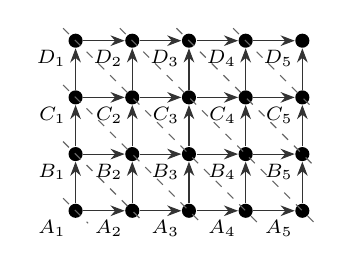
\begin{tikzpicture}[
  dot/.style={circle,fill,inner sep=1.8pt},
  edge/.style={-{Stealth[length=1.8mm]},black!80},
  every node/.style={font=\scriptsize},
  x=0.72cm,y=0.72cm
]
  \foreach \x in {1,...,5} {
    \foreach \y/\row in {1/A,2/B,3/C,4/D} {
      \node[dot] (p\x-\y) at (\x,\y) {};
      \node[anchor=north east] at (\x,\y) {$\row_{\x}$};
    }
  }
  \foreach \x [evaluate=\x as \nx using int(\x+1)] in {1,...,4} {
    \foreach \y in {1,...,4} \draw[edge] (p\x-\y)--(p\nx-\y);
  }
  \foreach \x in {1,...,5} {
    \foreach \y [evaluate=\y as \ny using int(\y+1)] in {1,...,3}
      \draw[edge] (p\x-\y)--(p\x-\ny);
  }
  \foreach \d in {2,...,8}
    \draw[dashed,black!60] ({max(1,\d-4)-0.22},{min(4,\d-1)+0.22}) --
      ({min(5,\d-1)+0.22},{max(1,\d-5)-0.22});
\end{tikzpicture}
\end{center}
\[
  s_{k-1}=
  \begin{cases}
    s_k-1+u_k, & k\le \mathit{row},\\
    s_k+u_k, & k>\mathit{row},
  \end{cases}
\]
trong đó \(\mathit{row}\) là số hàng theo chiều dọc của bản đồ.

Ta thấy phương trình chuyển trạng thái này phải chia hai trường hợp theo giá
trị của \(k\), nên có vẻ rất phiền. Tương ứng, khi đưa nó vào phương trình
quy hoạch để cài đặt, thuật toán cũng rườm rà. Vì vậy khi cài đặt, nói chung
ta không làm như vậy, mà thay bằng cách dưới đây:
\[
\begin{array}{ccccc}
D1&D2&D3&D4&D5\\
C1&C2&C3&C4&C5\\
B1&B2&B3&B4&B5\\
A1&A2&A3&A4&A5
\end{array}
\]

Đánh số các điểm trong bản đồ một cách quy tắc như trên, ta được phương trình
quy hoạch:
\[
  f_{i,j}=\min
  \begin{cases}
    f_{i-1,j}+\operatorname{Distance}((i-1,j),(i,j)),\\
    f_{i,j-1}+\operatorname{Distance}((i,j-1),(i,j)).
  \end{cases}
\]
Ở đây \(\operatorname{Distance}\) biểu thị độ dài cạnh giữa hai điểm kề nhau.

Cách làm này quả thật đơn giản hơn cách trên rất nhiều, nhưng nó đã phá vỡ
diện mạo vốn có của quy hoạch động, vì không còn đặc trưng giai đoạn rõ ràng.
Nếu nói cách này chia giai đoạn theo hàng của bản đồ \(A,B,C,D\), thì
``chuyển trạng thái'' của nó không hoàn toàn diễn ra giữa hai giai đoạn.

Có lẽ điều này không đáng kể, vì thực hành có sức thuyết phục hơn lý thuyết.
Nhưng nếu ta mở rộng đề bài: trong bản đồ, tìm hai đường đi từ góc trái dưới
đến góc phải trên, sao cho hai đường đi không dùng chung bất cứ cạnh nào và
tổng độ dài của hai đường là ngắn nhất. Khi ấy, dùng lại cách ``đơn giản''
này sẽ không dễ.

Nếu cứ gượng áp dụng cách này, hàm chỉ tiêu tối ưu sẽ cần chỉ số bốn chiều,
và rất khó xử lý ràng buộc hai đường đi ``không trùng cạnh''.

Quay lại phương pháp quy hoạch động ``chuẩn'' ban đầu, ta sẽ thấy bài toán
này rất dễ giải: chỉ cần thêm một chiều trạng thái. Dùng
\(s_k=(a_k,b_k)\) để lần lượt biểu thị vị trí của hai đường đi khi đã đi đến
giai đoạn \(k\). Tương ứng, biến quyết định cũng tăng thêm một chiều:
\(u_k=(x_k,y_k)\), lần lượt biểu thị hướng đi của hai đường. Khi chuyển trạng
thái, xét riêng từng đường:
\[
\begin{cases}
a_{k-1}=a_k-1+x_k,\quad b_{k-1}=b_k-1+y_k, & k\le \mathit{row},\\
a_{k-1}=a_k+x_k,\quad b_{k-1}=b_k+y_k, & k>\mathit{row}.
\end{cases}
\]

Khi viết phương trình quy hoạch, chỉ cần xử lý nhẹ trường hợp hai đường đi
đến cùng một điểm để giảm số quyết định có thể chọn:
\[
f_k(s_k)=
\begin{cases}
\displaystyle
\min_{u_k=(0,1),(1,0)}
\bigl(f_{k-1}(T_k(s_k,u_k))+\text{độ dài hai cạnh}\bigr),
& a_k=b_k,\\[0.8em]
\displaystyle
\min_{u_k=(0,0),(0,1),(1,0),(1,1)}
\bigl(f_{k-1}(T_k(s_k,u_k))+\text{độ dài hai cạnh}\bigr),
& a_k\ne b_k.
\end{cases}
\]

Từ ví dụ này có thể rút ra một kỹ thuật khi thiết kế thuật toán quy hoạch
động: chuyển trạng thái nói chung nên diễn ra giữa hai giai đoạn kề nhau
đôi khi cũng có thể giữa hai giai đoạn không kề nhau, nhưng cố gắng tránh
chuyển trạng thái trong cùng một giai đoạn.

Quy hoạch động là một phương pháp giải bài rất linh hoạt; trong thiết kế
thuật toán quy hoạch động còn nhiều kỹ thuật tương tự. Muốn nắm được các kỹ
thuật ấy có hai con đường: một là hiểu sâu bản chất của quy hoạch động, đó
cũng là lý do ngay từ đầu ta đã bàn về bản chất của nó; hai là thực hành
nhiều, không chỉ giải nhiều bài mà còn phải biết tìm quy luật và tổng kết kỹ
thuật từ quá trình giải bài.

\section{So sánh quy hoạch động với một số thuật toán}

Quy hoạch động là một trong nhiều phương pháp giải bài, nên tất nhiên có
nhiều liên hệ với một số thuật toán khác. Từ các liên hệ ấy, ta cũng có thể
nhìn ra một số đặc điểm của quy hoạch động.

\subsection{Quy hoạch động và truy hồi}

\paragraph{Quy hoạch động là thuật toán tối ưu hóa.}
Do ``danh tiếng'' của quy hoạch động quá lớn, nhiều người, thậm chí cả một số
tài liệu, thường coi một thuật toán rất giống quy hoạch động là quy hoạch
động. Thuật toán đó là truy hồi. Thực ra hai thuật toán này vẫn rất dễ phân
biệt.

Nếu chia theo mục tiêu giải bài, đề thi tin học chủ yếu có bốn loại: bài toán
phán định, bài toán xây dựng, bài toán đếm và bài toán tối ưu hóa. Trong thi
đấu, ta gặp nhiều nhất là bài toán tối ưu hóa, mà quy hoạch động chính là vũ
khí mạnh để giải các bài toán tối ưu hóa; do đó vị trí của quy hoạch động
trong thi đấu ngày càng cao. Còn phương pháp truy hồi cũng là một công cụ
mạnh khi xử lý bài toán phán định và bài toán đếm. Sau đây, qua hai ví dụ, ta
nói về mối liên hệ giữa truy hồi và quy hoạch động ở hai phương diện này.

\paragraph{Ví dụ 4. Bài toán đường đi tối ưu modulo 4.}
Trong đồ thị dưới đây, hãy tìm một đường đi từ đỉnh 1 đến đỉnh 4 sao cho số
dư của độ dài đường đi modulo 4 là nhỏ nhất.

\[
\begin{array}{c@{\quad}c@{\quad}c@{\quad}c}
1 & 2 & 3 & 4\\
\multicolumn{4}{c}{
\text{giữa các cặp đỉnh kề có các cạnh độ dài }
(3,1,0),\ (1,2,2),\ (2,3)
}
\end{array}
\]

Đây là một đồ thị nhiều tầng, hơn nữa là một đồ thị nhiều tầng đặc biệt. Tuy
hình thức của đồ thị đơn giản hơn đồ thị nhiều tầng thông thường, bài toán
đường đi tối ưu này lại không thể làm bằng quy hoạch động. Vì một đường đi
tối ưu từ đỉnh 1 đến đỉnh 4, khi đi đến đỉnh 2 hoặc đỉnh 3, số dư của độ dài
đường đi modulo 4 chưa chắc là nhỏ nhất. Nói cách khác, chiến lược con của
chiến lược tối ưu chưa chắc tối ưu; bài toán này không thỏa nguyên lý tối ưu.

Nhưng ta có thể chuyển nó thành bài toán phán định và dùng truy hồi để giải.
Ký hiệu \(f_k(s_k)\) là việc có tồn tại hay không một đường đi từ đỉnh 1 đến
đỉnh \(k\) có độ dài modulo 4 bằng \(s_k\). Công thức truy hồi là:
\[
f_1(s_1)=
\begin{cases}
\text{true}, & s_1=0,\\
\text{false}, & s_1=1,2,3,
\end{cases}
\]
là điều kiện biên, và
\[
f_k(s_k)=
f_{k-1}((s_k-\mathit{len}_{k,1})\bmod 4)
\vee
f_{k-1}((s_k-\mathit{len}_{k,2})\bmod 4)
\vee
f_{k-1}((s_k-\mathit{len}_{k,3})\bmod 4).
\]
Ở đây \(\mathit{len}_{k,i}\) biểu thị độ dài cạnh thứ \(i\) giữa đỉnh
\(k-1\) và đỉnh \(k\); dấu \(\vee\) biểu thị phép ``hoặc''.

Kết quả cuối cùng là giá trị \(s_4\) nhỏ nhất làm cho \(f_4(s_4)\) là đúng.

Công thức truy hồi này rất giống phương trình quy hoạch của quy hoạch động;
ở đây ta mượn ký hiệu của quy hoạch động cũng là để thể hiện rõ điểm ấy. Thực
ra tư tưởng của chúng cũng rất giống nhau: có thể nói truy hồi đã mượn tư
tưởng của quy hoạch động để giải một bài toán mà quy hoạch động không giải
được.

Một số bài toán quyết định nhiều giai đoạn, như bài này có đặc trưng giai
đoạn rất rõ, nhưng do không thỏa các tiền đề để dùng quy hoạch động như
nguyên lý tối ưu nên không thể áp dụng quy hoạch động. Khi đó có thể đưa giá
trị của hàm chỉ tiêu tối ưu vào phần chỉ số như một ``trạng thái'', biến bài
toán tối ưu hóa thành bài toán phán định, rồi mượn tư tưởng quy hoạch động và
dùng truy hồi để giải.

\paragraph{Ví dụ 5. Đinh và bóng (NOI 1999).}
Đề bài xem ở phụ lục.

Nhìn bài này rất dễ liên tưởng đến một bài quy hoạch động kinh điển. Trước
hết ta nhắc lại bài toán ấy.

\paragraph{Tam giác số (IOI 1994).}
Trong tam giác dưới đây, tìm một đường đi từ đỉnh trên xuống một vị trí ở
đáy, sao cho tổng các số đi qua là lớn nhất; mỗi bước chỉ được đi xuống trái
hoặc xuống phải.
\[
\begin{array}{ccccc}
&&7&&\\
&3&&8&\\
8&&1&&0\\
2&&7&&4\quad 4\\
4&&5&&2\quad 6\quad 5
\end{array}
\]

Trong bài này, ta chia giai đoạn theo số hàng đã đi qua, lấy vị trí ở mỗi
hàng làm trạng thái; quyết định là đi xuống trái, ký hiệu \(0\), hoặc xuống
phải, ký hiệu \(1\).

Phương trình chuyển trạng thái:
\[
  s_{k-1}=s_k-u_k.
\]

Phương trình quy hoạch:
\[
  f_k(s_k)=\max_{u_k=0,1} f_{k-1}(s_k-u_k)+\operatorname{Data}_k(s_k).
\]

Điều kiện biên:
\[
  f_k(0)=0,\qquad f_k(k+1)=0
  \qquad (0\le k\le \text{tổng số hàng}).
\]

Đây là một bài toán tối ưu hóa tương đối đơn giản. Ta còn có thể đổi nó
thành một bài toán đếm số nguyên đơn giản hơn: tính tổng số đường đi từ đỉnh
trên đến từng điểm. Ký hiệu tổng số này là \(f_k(s_k)\), khi đó công thức
truy hồi là:
\[
  f_k(s_k)=\sum_{u_k=0}^{1} f_{k-1}(s_k-u_k).
\]
Ở đây tuy công thức tổng chỉ có hai hạng, ta vẫn dùng ký hiệu \(\sum\) để làm
nổi bật sự giống nhau giữa công thức truy hồi này và phương trình quy hoạch ở
trên. Điều kiện biên của hai công thức hoàn toàn giống nhau.

Quay lại bài ``đinh và bóng'' ở trên, đây là một bài toán thống kê xác suất.
Tiếp tục dùng tư tưởng trên, ký hiệu \(f_k(s_k)\) là xác suất để bóng rơi vào
đinh thứ \(s_k\) ở hàng \(k\), ta có công thức truy hồi:
\[
\begin{aligned}
f_k(s_k)=&
\sum_{u_k=0}^{1}
\frac{f_{k-1}(s_k-u_k)\operatorname{Exist}_{k-1}(s_k-u_k)}{2}\\
&\quad+
f_{k-2}(s_k-1)\bigl(1-\operatorname{Exist}_{k-2}(s_k-1)\bigr).
\end{aligned}
\]
Trong đó hàm \(\operatorname{Exist}_k(s_k)\) biểu thị đinh thứ \(s_k\) ở
hàng \(k\) có tồn tại hay không; tồn tại thì lấy giá trị \(1\), không tồn tại
thì lấy \(0\).

Điều kiện biên:
\[
  f_1(1)=1,\qquad
  f_k(0)=0,\qquad f_k(k+1)=0
  \qquad (1\le k\le \text{tổng số hàng}).
\]

Có thể thấy công thức này tuy hơi khác hai công thức trên, nhưng tư tưởng cơ
bản vẫn tương tự. Trong quá trình giải bài này, ta lại vận dụng tư tưởng của
quy hoạch động.

Nói chung, nhiều bài toán tối ưu hóa có bài toán đếm tương ứng; ngược lại,
nhiều bài toán đếm cũng có bài toán tối ưu hóa tương ứng. Vì vậy khi gặp hai
loại bài này, ta có thể liên hệ và phát triển thêm, suy rộng từ một bài sang
nhiều bài, từ so sánh mà hiểu sâu hơn tư tưởng quy hoạch động.

Thực ra tư tưởng của truy hồi và quy hoạch động vốn rất giống nhau, cũng
không cần nói ai mượn tư tưởng của ai. Mấu chốt là ta phải nắm được tư tưởng
ấy; như vậy, dù dùng quy hoạch động để giải bài tối ưu hóa hay dùng truy hồi
để giải bài phán định, bài đếm, ta đều có thể xử lý thành thạo.

\subsection{Quy hoạch động và tìm kiếm}

\paragraph{Quy hoạch động là thuật toán hiệu suất cao, chi phí cao.}
Cùng là giải bài toán tối ưu hóa, có bài ta dùng quy hoạch động, có bài lại
cần dùng tìm kiếm. Trong đó có quy luật gì không?

Ta biết rằng nếu tạm bỏ qua yếu tố hiệu suất thời gian và không gian, trong
các thuật toán giải bài tối ưu hóa, có thể nói tìm kiếm là ``vạn năng''. Vì
vậy, bài toán mà quy hoạch động giải được thì tìm kiếm cũng nhất định giải
được.

Việc viết lại một thuật toán quy hoạch động thành tìm kiếm rất thuận tiện:
phương trình chuyển trạng thái, phương trình quy hoạch và điều kiện biên đều
có thể ``cấy ghép'' trực tiếp; khác biệt chỉ là thứ tự giải. Quy hoạch động
là truy hồi từ dưới lên, còn tìm kiếm là đệ quy từ trên xuống; ở đây nói đến
tìm kiếm theo chiều sâu, tìm kiếm theo chiều rộng cũng tương tự.

Ngược lại, ta cũng có thể viết lại thuật toán tìm kiếm thành quy hoạch động.
Tìm kiếm không gian trạng thái thực chất là liệt kê các đỉnh trong một đồ thị
ẩn; phép liệt kê này là từ trên xuống. Nếu đảo ngược thứ tự liệt kê thành từ
dưới lên thì nó trở thành quy hoạch động. Tất nhiên ở đây có một điều kiện:
các đỉnh trong đồ thị ẩn phải có thể sắp thứ tự, điều này sẽ được nói rõ hơn
ở phần sau.

Chính vì quy hoạch động và tìm kiếm khác nhau ở thứ tự giải, nên hiệu suất
thời gian của chúng cũng khác nhau. Trong tìm kiếm thường xuất hiện tình
huống sau:
\[
\begin{array}{ccc}
\text{(a) đồ thị ẩn} & \text{(b) cây tìm kiếm} & \text{(c) quy hoạch động}\\
\begin{array}{c}
A_1\\
B_1\quad B_2\\
C_1\quad C_2\quad C_3
\end{array}
&
\begin{array}{c}
A_1\\
B_1\quad B_2\\
C_1\quad C_2\quad C_2\quad C_3
\end{array}
&
\begin{array}{c}
A_1\\
B_1\quad B_2\\
C_1\quad C_2\quad C_3
\end{array}
\end{array}
\]

Đối với một đồ thị ẩn gồm vài trạng thái như hình (a), dùng tìm kiếm sẽ có
lặp lại như hình (b), trạng thái \(C_2\) bị tìm hai lần. Trong tìm kiếm theo
chiều sâu, sự lặp lại này sẽ làm lặp cả cây con tìm kiếm lấy \(C_2\) làm
gốc; trong tìm kiếm theo chiều rộng, tuy sự lặp này có thể bị loại ngay,
nhưng chi phí thời gian cũng không nhỏ. Quy hoạch động thì không có vấn đề
này, như hình (c).

Nói chung, ưu thế hiệu suất thời gian của quy hoạch động là điều tìm kiếm khó
sánh được. Tất nhiên với một số bài, hoàn toàn không xuất hiện trạng thái lặp
lại, khi ấy tốc độ của tìm kiếm và quy hoạch động không khác nhau. Về lý
thuyết, mọi thuật toán tìm kiếm trên đồ thị ẩn có thứ tự tô-pô, mà trong thực
tế điều kiện này thường có thể thỏa, đều có thể viết lại thành quy hoạch
động. Nhưng trên thực tế, trong nhiều trường hợp ta vẫn buộc phải dùng thuật
toán tìm kiếm. Vậy cài đặt quy hoạch động còn trở ngại gì?

\[
\begin{array}{ccc}
\text{(a) đồ thị ẩn} & \text{(b) tìm kiếm} & \text{(c) quy hoạch động}\\
\begin{array}{c}
A_1\\
B_1\quad B_2\\
C_1\quad C_2\quad C_3
\end{array}
&
\begin{array}{c}
A_1\\
B_1\quad B_2\\
\phantom{C_1\quad}C_2\quad C_2
\end{array}
&
\begin{array}{c}
A_1\\
B_1\quad B_2\\
C_1\quad C_2\quad C_3
\end{array}
\end{array}
\]

Xét đồ thị ẩn ở hình (a), trong đó có hai trạng thái không thể đạt được từ
trạng thái ban đầu. Trong thuật toán tìm kiếm, hai trạng thái như vậy sẽ
không được xét, như hình (b). Nhưng do quy hoạch động giải từ dưới lên, nó
không thể ước lượng điều này, nên phải duyệt toàn bộ trạng thái, như hình
(c).

Nói chung, quy hoạch động luôn phải duyệt mọi trạng thái, còn tìm kiếm có thể
loại bỏ một số trạng thái vô hiệu. Quan trọng hơn, tìm kiếm còn có thể cắt
tỉa, có khả năng cắt bỏ rất nhiều trạng thái không cần thiết; vì vậy chi phí
không gian thường thấp hơn quy hoạch động rất nhiều.

Làm thế nào để điều hòa mâu thuẫn giữa hiệu suất cao và chi phí cao của quy
hoạch động? Một cách chiết trung là thuật toán ghi nhớ. Khi giải, thuật toán
ghi nhớ vẫn theo thứ tự từ trên xuống, nhưng mỗi khi giải xong một trạng thái
thì lưu lời giải của nó lại; về sau gặp lại trạng thái này thì không cần giải
lại. Cách này tổng hợp ưu điểm của cả tìm kiếm và quy hoạch động, nên có giá
trị thực dụng cao.

\subsection{Quy hoạch động và luồng mạng}

\paragraph{Quy hoạch động là thuật toán dễ thiết kế, dễ cài đặt.}
Do quan hệ trong đồ thị phức tạp và không có thứ tự, nói chung khó thể hiện
đặc trưng giai đoạn, ngoại trừ các đồ thị đặc biệt như đồ thị nhiều tầng hoặc
cách phân đoạn đặc biệt như Floyd; vì vậy quy hoạch động không được ứng dụng
nhiều trong lý thuyết đồ thị. Nhưng có một lớp đồ thị mà các đỉnh có thứ tự:
đó là đồ thị có hướng không chu trình.

Trong đồ thị có hướng không chu trình, ta có thể sắp xếp tô-pô các đỉnh để
làm nổi bật đặc trưng có thứ tự, từ đó chia giai đoạn. Thuật toán tìm đường
đi ngắn nhất trong đồ thị có hướng không chu trình~\cite{modern-algorithms}
đã thể hiện tư tưởng quy hoạch động đơn giản. Nhưng quy hoạch động còn có
ứng dụng giá trị hơn trong lý thuyết đồ thị. Trước hết xét một ví dụ.

\paragraph{Ví dụ 6. Bài toán đường phố cho \(N\) người.}
Trong bài toán đường phố ở ví dụ 3, nếu có \(N\) người cần đi từ góc trái
dưới đến góc phải trên, yêu cầu tổng độ dài các cạnh mà họ đi qua là lớn
nhất. Tất nhiên, ở đây mỗi người cũng chỉ được đi sang phải hoặc đi lên. Dưới
đây là một mẫu trong bản gốc: hình trái là ba đường đi từ điểm xuất phát đến
đích, hình phải là các cạnh họ đã đi qua. Tổng độ dài các cạnh này là
\[
5+4+3+6+3+3+5+8+8+7+4+5+9+5+3=78,
\]
không nhất định là lớn nhất.

Bài này là một mở rộng nữa của bài toán đường phố. Mô phỏng cách giải bài
đường phố, ta vẫn có thể dùng quy hoạch động để giải bài này. Nhưng lần này
\(N\) người đi đồng thời, nên biến trạng thái cần dùng \(N\) chiều để biểu
diễn. Tương ứng, biến quyết định cũng phải trở thành \(N\) chiều,
\[
  u_k=(u_{k,1},u_{k,2},\ldots,u_{k,N}).
\]
Phương trình chuyển trạng thái không cần thay đổi nhiều:
\[
\begin{cases}
s_{k-1,i}=s_{k,i}-1+u_{k,i}, & k\le \mathit{row},\\
s_{k-1,i}=s_{k,i}+u_{k,i}, & k>\mathit{row},
\end{cases}
\qquad 1\le i\le N.
\]

Khi viết phương trình quy hoạch, cần chú ý cách tính tổng độ dài các cạnh mà
\(N\) đường đi đi qua ở giai đoạn \(k\). Ở đây dùng \(g_k(s_k,u_k)\) để biểu
diễn:
\[
  f_k(s_k)=
  \max_{u_{k,i}=0,1\ (1\le i\le N)}
  \bigl(f_{k-1}(T_k(s_k,u_k))+g_k(s_k,u_k)\bigr).
\]
Điều kiện biên là
\[
  f_1((1,1,\ldots,1))=0.
\]

Có thể thấy, về mặt lý thuyết, việc chuyển thuật toán quy hoạch động ban đầu
sang bài toán này hoàn toàn khả thi. Nhưng độ phức tạp thời gian và không
gian của thuật toán quy hoạch động hiện tại đã là hàm mũ theo \(N\); chỉ cần
\(N\) hơi lớn, thuật toán này đã không thể cài đặt.

Bây giờ đổi một góc nhìn khác: xem \(N\) đường đi là một luồng có lưu lượng
\(N\) trong mạng. Mục tiêu giải bài khi đó là làm cho chi phí của luồng này
lớn nhất. Nhưng bài này lại khác bài toán luồng chi phí thông thường: trên
mỗi cạnh \(e\), chi phí luồng không phải là tích giữa lưu lượng và trọng số
\(f(e)w(e)\), mà được tính theo công thức
\[
\begin{cases}
w(e), & f(e)>0,\\
0, & f(e)=0.
\end{cases}
\]

Để thuật toán luồng chi phí kinh điển áp dụng được cho bài này, ta cần biến
đổi mô hình một chút. Mỗi cạnh có trọng số \(w_0\) được tách thành hai cạnh
song song:
\[
\begin{array}{c}
c_1=1,\quad w_1=w_0,\\
c_2=\infty,\quad w_2=0.
\end{array}
\]
Sau khi tách, một cạnh có trọng số nhưng sức chứa bị giới hạn là \(1\); cạnh
còn lại không giới hạn sức chứa, nhưng đi qua cạnh này thì không được tính
chi phí. Như vậy ta đã chuyển bài toán thành một bài toán luồng cố định chi
phí cực đại chuẩn.

Thuật toán này có thể dùng thuật toán luồng cực đại chi phí nhỏ nhất kinh
điển, ở đây không nói chi tiết; xem chương trình nguồn trong phụ lục.

Ví dụ này do tác giả mô phỏng bài ``máy dò chướng ngại vật'' của IOI
1997~\cite{detector-statement} mà đặt ra. Bài ``máy dò chướng ngại vật''
phức tạp hơn bài này, nhưng tư tưởng cơ bản tương tự. Các bài tương tự còn có
``cải tạo mê cung'' trong trại mùa đông năm 1999~\cite{maze}. Từ những bài
này đều có thể thấy liên hệ giữa quy hoạch động và luồng mạng.

Mở rộng ra trường hợp tổng quát, mọi bài toán luồng chi phí trong đồ thị có
hướng không chu trình, về lý thuyết, đều có thể giải bằng quy hoạch động.
Đối với bài toán luồng chi phí có lưu lượng \(N\), nếu lưu lượng không cố
định thì \(N\) cần được tính trước, dùng biến \(N\) chiều
\[
  s_k=(s_{k,1},s_{k,2},\ldots,s_{k,N})
\]
để mô tả trạng thái, trong đó \(s_{k,i}\in V\) với \(1\le i\le N\). Tương ứng,
quyết định cũng được biểu diễn bằng biến \(N\) chiều
\[
  u_k=(u_{k,1},u_{k,2},\ldots,u_{k,N}),
\]
trong đó \(u_{k,i}\in E(s_{k,i})\) với \(1\le i\le N\), và \(E(v)\) biểu thị
tập các cung đi vào \(v\). Khi đó phương trình chuyển trạng thái có thể viết:
\[
  s_{k-1,i}=\text{đỉnh đuôi của cung }u_{k,i}.
\]
Phương trình quy hoạch là
\[
  f_k(s_k)=
  \operatorname*{opt}_{u_{k,i}\in E(s_{k,i})}
  \left(f_k(T_k(s_k,u_k))+\sum_{i=1}^{N} w(u_{k,i})\right).
\]
Điều kiện biên là
\[
  f_1((1,1,\ldots,1))=0.
\]

Nhưng vì thuật toán quy hoạch động là thuật toán cấp mũ, nó bị hạn chế rất
lớn trong cài đặt, chỉ dùng được cho một số bài có \(N\) rất nhỏ. Tuy nhiên
trong giải bài thi, chẳng hạn các bài IOI 1997 và kiểm tra trại mùa đông 1999
nói trên, khuynh hướng dùng quy hoạch động của chúng ta rất rõ. Trong bài
``máy dò chướng ngại vật'', ta dùng chiến lược tham lam, tìm lời giải tối ưu
cục bộ khi \(N=1\) hoặc \(N=2\)~\cite{detector-solution}. Điều này chủ yếu có
hai nguyên nhân:

\begin{enumerate}
  \item Tuy luồng mạng có thuật toán kinh điển, trong thi đấu không thể xuất
  hiện bài toán kinh điển nguyên dạng. Nếu muốn dùng thuật toán luồng mạng,
  cần trải qua một quá trình biến đổi mô hình; đôi khi phép biến đổi này khá
  khó. Vì vậy, về mặt thiết kế thuật toán, quy hoạch động linh hoạt và khéo
  léo lại đơn giản hơn.

  \item Thuật toán luồng mạng cài đặt rườm rà, điều này được thừa nhận rộng
  rãi. Vì thế trong môi trường thi đấu căng thẳng, thuật toán quy hoạch động
  vốn có một khuôn mẫu nhất định khi cài đặt lại có thêm một tầng ưu thế.
\end{enumerate}

Chính vì quy hoạch động đơn giản trong thiết kế và cài đặt, nên khi \(N\)
không quá lớn, tức khi quy hoạch động khả thi, ta vẫn nên cố gắng dùng quy
hoạch động.

\section{Kết luận}

Nội dung bài viết này khá tạp, là sự lĩnh hội, hiểu biết và kinh nghiệm của
tác giả về quy hoạch động trong vài năm. Tuy phần lớn dung lượng nói về lý
thuyết, mục đích căn bản vẫn là hướng dẫn thực hành.

Theo tác giả, quy hoạch động là một lớp phương pháp giải bài linh hoạt nhất
và thể hiện trình độ người giải rõ nhất trong thi tin học hiện nay. Nội dung
bài viết tuy nhiều, nhưng chưa thể bao quát dù chỉ một phần nhỏ của quy hoạch
động. ``Điều học được trên giấy rốt cuộc vẫn nông; muốn biết chắc việc này
phải tự mình làm.'' Muốn thật sự lĩnh hội, hiểu tư tưởng quy hoạch động và
nắm được kỹ thuật giải bài bằng quy hoạch động, cần không ngừng đào sâu, tìm
tòi trong thực hành. Thực hành nhiều rồi, tự nhiên sẽ cảm nhận được cái hay
của việc dần bước vào cảnh giới tốt hơn.

\begin{center}
Quy hoạch động,\\
lẽ thường của thuật toán,\\
cái hay khi vận dụng,\\
nằm ở một lòng.
\end{center}

\appendix
\section{Một số đề bài và chương trình nguồn}

\subsection{Đề bài ``Bố trí cửa sổ tiệm hoa''}

\paragraph{Little Shop of Flowers.}

\paragraph{Bài toán.}
Bạn muốn bố trí cửa sổ của tiệm hoa theo cách đẹp mắt nhất. Bạn có \(F\) bó
hoa, mỗi bó thuộc một loài khác nhau, và có ít nhất từng ấy bình hoa xếp
thành một hàng. Các bình được gắn cố định trên giá và được đánh số liên tiếp
từ \(1\) đến \(V\), trong đó \(V\) là số bình, từ trái sang phải; bình \(1\)
là bình ngoài cùng bên trái, bình \(V\) là bình ngoài cùng bên phải. Các bó
hoa có thể di chuyển và được nhận diện duy nhất bằng các số nguyên từ \(1\)
đến \(F\). Các số này có ý nghĩa: chúng xác định thứ tự bắt buộc của các bó
hoa trong hàng bình, sao cho bó hoa \(i\) phải nằm trong một bình ở bên trái
bình chứa bó hoa \(j\) mỗi khi \(i<j\). Chẳng hạn, bạn có một bó đỗ quyên
(mã số \(1\)), một bó thu hải đường (mã số \(2\)) và một bó cẩm chướng (mã số
\(3\)). Khi đó mọi bó hoa phải được đặt vào bình theo đúng thứ tự mã số: bó
đỗ quyên phải ở bên trái bó thu hải đường, và bó thu hải đường phải ở bên
trái bó cẩm chướng. Nếu số bình nhiều hơn số bó hoa thì các bình thừa sẽ để
trống. Mỗi bình chỉ chứa được một bó hoa.

Mỗi bình có một đặc tính riêng, giống như mỗi loài hoa cũng vậy. Do đó, đặt
một bó hoa vào một bình sẽ tạo ra một giá trị thẩm mỹ nhất định, biểu diễn
bằng một số nguyên. Các giá trị thẩm mỹ được cho trong một bảng như dưới đây.
Để trống một bình có giá trị thẩm mỹ \(0\).

\[
\begin{array}{c|rrrrr}
 & \multicolumn{5}{c}{\text{Bình}}\\
\text{Bó hoa} & 1&2&3&4&5\\ \hline
1\ (\text{đỗ quyên}) & 7&23&-5&-24&16\\
2\ (\text{thu hải đường}) & 5&21&-4&10&23\\
3\ (\text{cẩm chướng}) & -21&5&-4&-20&20
\end{array}
\]

Theo bảng, chẳng hạn đỗ quyên sẽ rất đẹp trong bình \(2\), nhưng rất tệ trong
bình \(4\).

Để đạt hiệu quả đẹp mắt nhất, bạn phải cực đại hóa tổng giá trị thẩm mỹ của
cách bố trí, đồng thời giữ đúng thứ tự bắt buộc của các bó hoa. Nếu có hơn
một cách bố trí đạt tổng lớn nhất, bất kỳ cách nào trong số đó đều được chấp
nhận. Bạn phải xuất đúng một cách bố trí.

\paragraph{Giả thiết.}
\[
1\le F\le 100,
\]
trong đó \(F\) là số bó hoa; các bó hoa được đánh số từ \(1\) đến \(F\).
\[
F\le V\le 100,
\]
trong đó \(V\) là số bình.
\[
-50\le A_{ij}\le 50,
\]
trong đó \(A_{ij}\) là giá trị thẩm mỹ khi đặt bó hoa \(i\) vào bình \(j\).

\paragraph{Dữ liệu vào.}
Dữ liệu vào là tệp văn bản \texttt{flower.inp}. Dòng đầu chứa hai số
\(F,V\). \(F\) dòng tiếp theo: mỗi dòng chứa \(V\) số nguyên, sao cho
\(A_{ij}\) là số thứ \(j\) trên dòng thứ \(i+1\) của tệp vào.

\paragraph{Dữ liệu ra.}
Dữ liệu ra phải là tệp văn bản \texttt{flower.out} gồm hai dòng. Dòng đầu
chứa tổng giá trị thẩm mỹ của cách bố trí. Dòng thứ hai trình bày cách bố trí
dưới dạng danh sách \(F\) số, sao cho số thứ \(k\) trên dòng này cho biết
bình chứa bó hoa \(k\).

\paragraph{Ví dụ.}
\begin{verbatim}
flower.inp:
3 5
7 23 -5 -24 16
5 21 -4 10 23
-21 5 -4 -20 20

flower.out:
53
2 4 5
\end{verbatim}

\paragraph{Chấm điểm.}
Chương trình được phép chạy trong 2 giây. Không có điểm từng phần cho một ca
kiểm thử.

\subsection{Đề bài ``Đinh và bóng''}

Có một tấm gỗ hình tam giác đặt thẳng đứng, trên đó đóng \(n(n+1)/2\) chiếc
đinh, và có \(n+1\) ô chứa bóng. Khi \(n=5\), bố cục như Hình 1. Mỗi đinh
cách các đinh xung quanh một khoảng \(d\); bề rộng của mỗi ô cũng bằng \(d\).
Ngoài ô ngoài cùng bên trái và ngoài cùng bên phải, mỗi ô đều nằm thẳng dưới
khe giữa hai đinh ở hàng dưới cùng.

Thả cho tâm của một quả bóng có đường kính hơi nhỏ hơn \(d\) nằm đúng trên
đinh trên cùng rồi lăn tự do trên tấm gỗ. Mỗi khi chạm một đinh, bóng có thể
rơi sang trái hoặc sang phải với xác suất đều bằng \(1/2\), và tâm bóng sẽ
đúng hướng đến đinh tiếp theo mà nó sắp chạm. Hình 2 là một đường đi có thể
của bóng.

Ta biết xác suất bóng rơi vào ô thứ \(i\) là
\[
  p_i=C_n^i 2^{-n}=\frac{n!}{i!(n-i)!2^n},
\]
trong đó \(i\) là số hiệu ô, đánh số từ trái sang phải là \(0,1,\ldots,n\).

Bài toán hiện tại là tính xác suất \(p_m\) để bóng rơi vào ô mang số \(m\)
sau khi một số đinh bị nhổ đi. Giả sử hàng đinh dưới cùng không bị nhổ. Hình
3 là một đường đi có thể của bóng sau khi một số đinh bị nhổ.

\begin{center}
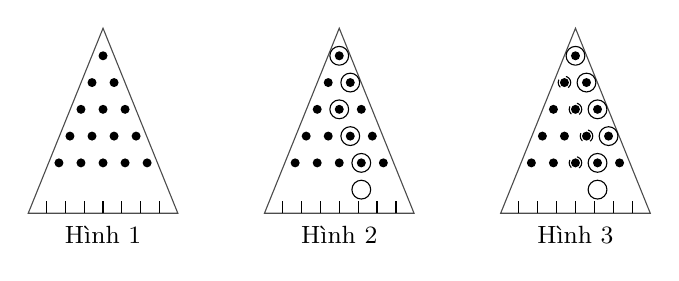
\begin{tikzpicture}[
  nail/.style={circle,fill,inner sep=1.15pt},
  gone/.style={circle,draw,dashed,inner sep=1.6pt},
  ball/.style={circle,draw,inner sep=2.4pt},
  every node/.style={font=\scriptsize},
  x=1cm,y=1cm
]
  \foreach \shift/\caption in {0/Hình 1,3.0/Hình 2,6.0/Hình 3} {
    \begin{scope}[shift={(\shift,0)}]
      \draw[black!70] (-0.95,0)--(0,2.35)--(0.95,0)--cycle;
      \foreach \r in {1,...,5} {
        \foreach \c in {1,...,\r} {
          \pgfmathsetmacro{\xx}{(\c-(\r+1)/2)*0.28}
          \pgfmathsetmacro{\yy}{2.0-(\r-1)*0.34}
          \node[nail] at (\xx,\yy) {};
        }
      }
      \foreach \i in {0,...,6} \draw (-0.72+\i*0.24,0.0)--(-0.72+\i*0.24,0.16);
      \node[font=\small] at (0,-0.28) {\caption};
    \end{scope}
  }

  \begin{scope}[shift={(3.0,0)}]
    \foreach \x/\y in {0/2.0,0.14/1.66,0.0/1.32,0.14/0.98,0.28/0.64,0.28/0.30}
      \node[ball] at (\x,\y) {};
  \end{scope}

  \begin{scope}[shift={(6.0,0)}]
    \foreach \x/\y in {-0.14/1.66,0/1.32,0.14/0.98,0.0/0.64}
      \node[gone] at (\x,\y) {};
    \foreach \x/\y in {0/2.0,0.14/1.66,0.28/1.32,0.42/0.98,0.28/0.64,0.28/0.30}
      \node[ball] at (\x,\y) {};
  \end{scope}
\end{tikzpicture}
\end{center}

\paragraph{Dữ liệu vào.}
Dòng 1 chứa hai số nguyên \(n\) và \(m\), với \(2\le n\le 50\) và
\(0\le m\le n\). \(n\) dòng tiếp theo lần lượt chứa thông tin của các hàng
đinh từ trên xuống dưới trên tấm gỗ. Trong mỗi dòng, ký tự \texttt{*} biểu
thị đinh còn ở đó, ký tự \texttt{.} biểu thị đinh đã bị nhổ. Chú ý rằng trong
\(n\) dòng này, ký tự khoảng trắng có thể xuất hiện ở bất kỳ vị trí nào.

\paragraph{Dữ liệu ra.}
Chỉ một dòng, là một phân số tối giản; \(0\) viết thành \texttt{0/1}. Đó là
xác suất \(p_m\) để bóng rơi vào ô mang số \(m\). Phân số tối giản được định
nghĩa như sau: \(A/B\) là phân số tối giản khi và chỉ khi \(A,B\) là các số
nguyên dương và \(A,B\) không có ước chung lớn hơn \(1\).

\paragraph{Ví dụ.}
\begin{verbatim}
Input:
5 2
*
*.
***
*.**
*****

Output:
7/16
\end{verbatim}

\subsection{Chương trình nguồn cách 1 cho ví dụ 2}

\begin{verbatim}
program IOI99_LittleShopOfFlowers;
var
    F,V :byte;    {number of flower bunches and vases}
    A :array [1..100,1..100] of shortint;    {A[i,j] aesthetic value}
    Best:array [0..100,0..100] of integer;
        {Best[i,j]: optimum for first i bunches, with i-th in vase j}
    Previous :array [1..100,1..100] of byte;
        {Previous[i,j]: position of bunch i-1 in the optimum for Best[i,j]}

procedure ReadIn;          {read input}
var
     i,j :byte;
begin
     reset(input);
     readln(F,V);
     for i:=1 to F do
     begin
           for j:=1 to V do
                 read(A[i,j]);
           readln;
     end;
     close(input);
end;

procedure Work; {main DP procedure}
var
     i,j,t :byte;
begin
     fillchar(Best[0],sizeof(Best[0]),0); {boundary condition}
     for i:=1 to F do
           for j:=i to V+i-F do
           begin
                 Best[i,j]:=low(Best[i,j]);
                 for t:=i-1 to j-1 do {enumerate the position of bunch i-1}
                       if Best[i-1,t]>Best[i,j] then
                       begin      {update current optimum}
                            Best[i,j]:=Best[i-1,t];
                            Previous[i,j]:=t;
                       end;
                 inc(Best[i,j],A[i,j]);
           end;
end;

procedure Print; {print optimum}
var
     i,j :byte;
     Put :array [1..100] of byte;
begin
     i:=F;
     for j:=F+1 to V do {choose global optimum}
           if Best[F,j]>Best[F,i] then
                i:=j; {i is the position of the last bunch}
     rewrite(output);
     writeln(Best[F,i]);
     for j:=F downto 1 do
     begin
           Put[j]:=i;
           i:=Previous[j,i];
     end;
     for i:=1 to F do
           write(Put[i],' ');
     writeln;
     close(output);
end;

begin
     assign(input,'flower.inp');
     assign(output,'flower.out');
     ReadIn;
     Work;
     Print;
end.
\end{verbatim}

\subsection{Chương trình nguồn cách 2 cho ví dụ 2}

\begin{verbatim}
program IOI99_LittleShopOfFlowers;
var
    F,V :byte;    {number of flower bunches and vases}
    A :array [1..100,1..100] of shortint;   {A[i,j] aesthetic value}
    Best:array [0..100,0..100] of integer;
        {Best[i,j]: optimum for first i bunches in first j vases}
    Choice :array [0..100,0..100] of boolean;
        {Choice[i,j]: whether bunch i is put in vase j}

procedure ReadIn;       {read input}
var
    i,j :byte;
begin
    reset(input);
    readln(F,V);
    for i:=1 to F do
    begin
          for j:=1 to V do
                read(A[i,j]);
          readln;
    end;
    close(input);
end;

procedure Work; {main DP procedure}
var
     i,j :byte;
begin
     fillchar(Best[0],sizeof(Best[0]),0); {boundary condition}
     for i:=1 to F do
     begin
           Best[i,i]:=Best[i-1,i-1]+A[i,i]; {the only choice}
           Choice[i,i]:=true;
           for j:=i+1 to V+i-F do
           begin
                 Choice[i,j]:=Best[i-1,j-1]+A[i,j]>Best[i,j-1];
                 if Choice[i,j]
                 then Best[i,j]:=Best[i-1,j-1]+A[i,j] {i in j}
                 else Best[i,j]:=Best[i,j-1]; {i not in j}
           end;
     end;
end;

procedure Print; {print optimum}
var
    i,j :byte;
    Put :array [1..100] of byte; {Put[i]: vase containing bunch i}
begin
    rewrite(output);
    writeln(Best[F,V]);
    i:=F;
    for j:=V downto 1 do {backtrack Put}
          if Choice[i,j] then
          begin
               Put[i]:=j;
               dec(i);
          end;
    for i:=1 to F do
    begin
         write(Put[i]);
         if i<F then write(' ');
    end;
    writeln;
    close(output);
end;

begin
     assign(input,'flower.inp');
     assign(output,'flower.out');
     ReadIn;
     Work;
     Print;
end.
\end{verbatim}

\subsection{Mở rộng ví dụ 3: tìm hai đường ngắn nhất không trùng cạnh}

\begin{verbatim}
program N_Street;
const
     MaxSize=90; {maximum map size}
type
     TPlanarArr=array [1..MaxSize,1..MaxSize] of integer;
var
     Row,Col :byte;         {number of rows and columns}
     Best,B1 :TPlanarArr; {current and previous stage optimum functions}
     Street :array [0..1] of TPlanarArr; {horizontal and vertical edges}

procedure ReadIn;        {read input}
var
    i,j :byte;
begin
    reset(input);
    readln(Row,Col);
    for i:=1 to Row do
    begin
          for j:=1 to Col-1 do
                read(Street[0,i,j]);
          readln;
    end;
    for j:=1 to Col do
    begin
          for i:=1 to Row-1 do
                read(Street[1,i,j]);
          readln;
    end;
    close(input);
end;

procedure Work; {DP procedure; unlike the article, this solves backward}
var
    k,        {stage}
    s1,s2, {state, two-dimensional}
    u1,u2, {decision, two-dimensional}
    t1,t2,    {previous-stage states derived from s and u}
    m,        {number of states in this stage}
    m1,m2 :byte;        {smaller and larger of Row and Col}
    e1,e2     :integer; {edge lengths corresponding to u1,u2}
    function GetET(s,u:byte; var e:integer; var t:byte):boolean; {get e,t}
    begin
         GetET:=false;
         if   (k>=Row) and (s=1) and (u=1) or
              (k>=Col) and (s=m) and (u=0) then
              exit; {out of bounds}
         GetET:=true;
         if k<Row {two cases according to k}
         then begin
              e:=Street[u,k+1-s,s];
              t:=s+1-u;
         end
         else begin
              e:=Street[u,Row+1-s,k-Row+s];
              t:=s-u;
         end;
    end;
begin
    if Row<Col
    then begin
         m1:=Row; m2:=Col;
    end
    else begin
         m1:=Col; m2:=Row;
    end;
    Best[1,1]:=0;
    for k:=Row+Col-2 downto 1 do {solve backward}
    begin
         if k<m1
         then m:=k
         else if k>m2
              then m:=Row+Col-k
              else m:=m1;
         B1:=Best;
         for s1:=1 to m do
              for s2:=1 to m do
              begin
                   Best[s1,s2]:=$7000; {initialize to a large value}
                   for u1:=0 to 1 do
                        if GetET(s1,u1,e1,t1) then
                             for u2:=0 to 1 do
                                  if ((s1<>s2) or (u1<>u2)) and
                                        GetET(s2,u2,e2,t2) and
                                        (B1[t1,t2]+e1+e2<Best[s1,s2]) then
                                        Best[s1,s2]:=B1[t1,t2]+e1+e2;
                                        {update optimum}
              end;
    end;
end;

begin
     assign(input,'input.txt');
     assign(output,'output.txt');
     ReadIn;
     Work;
     rewrite(output);
     writeln(Best[1,1]);
     close(output);
end.
\end{verbatim}

\subsection{Chương trình nguồn bài đường đi tối ưu modulo 4}

\begin{verbatim}
program BestPath_mod4;
const
    MaxN=100; {maximum number of vertices}
    MaxE=100; {maximum number of edges between two vertices}
var
    N :byte;       {number of vertices}
    E :array [1..MaxN,0..MaxE] of integer;
        {E[i,0]: number of edges between vertex i and i+1}
        {E[i,j]: length of the j-th edge between vertex i and i+1}
    Best:array [1..MaxN,0..3] of boolean;
        {Best[k,s]: path from 1 to k with length mod 4 = s exists}

procedure ReadIn;         {read input}
var
    i,j :byte;
begin
     reset(input);
     readln(N);
     for i:=1 to N-1 do
     begin
           read(E[i,0]);
           for j:=1 to E[i,0] do
                 read(E[i,j]);
           readln;
     end;
     close(input);
end;

procedure Work; {main recurrence}
var
     k,s,u      :byte;    {stage, state, decision}
begin
     fillchar(Best,sizeof(Best),false);
     Best[1,0]:=true; {boundary condition}
     for k:=2 to N do
           for s:=0 to 3 do
                for u:=1 to E[k-1,0] do
                     Best[k,s]:=Best[k,s] or Best[k-1,($10000+s-E[k-1,u]) mod 4];
                          {add 10000h to avoid a negative value}
end;

procedure Print; {only output the optimum path's value mod 4, not the path}
var
     i     :byte;
begin
     for i:=0 to 3 do
           if Best[N,i] then
                break;
     rewrite(output);
     writeln(i);
     close(output);
end;

begin
    assign(input,'input.txt');
    assign(output,'output.txt');
    ReadIn;
    Work;
    Print;
end.
\end{verbatim}

\subsection{Chương trình nguồn bài ``Đinh và bóng''}

\begin{verbatim}
{$A+,B-,D+,E+,F-,G+,I+,L+,N+,O-,P-,Q-,R-,S-,T-,V+,X+,Y+}
{$M 65520,0,655360}
program Ball;
var
    N,M :byte;
    Nail :array [1..50,1..50] of byte;
    Poss      :array [0..50,0..50] of comp;

procedure ReadIn;
var
     i,j :byte;
     c     :char;
begin
     reset(input);
     readln(N,M);
     for i:=1 to N do
           for j:=1 to i do
           begin
                 repeat
                       read(c);
                 until c in ['*','.'];
                 if c='*'
                 then Nail[i,j]:=1
                 else Nail[i,j]:=0;
           end;
     close(input);
end;

procedure Work;
var
    i,j :byte;
begin
    fillchar(Poss,sizeof(Poss),0);
    Poss[0,0]:=1;
    for i:=1 to N do
          Poss[0,0]:=Poss[0,0]*2;
    for i:=0 to N-1 do
          for j:=0 to i do
                if Nail[i+1,j+1]=0
                then Poss[i+2,j+1]:=Poss[i+2,j+1]+Poss[i,j]
                else begin
                      Poss[i+1,j]:=Poss[i+1,j]+Poss[i,j]/2;
                      Poss[i+1,j+1]:=Poss[i+1,j+1]+Poss[i,j]/2;
               end;
end;

procedure Print;
var
     a,b :comp;
begin;
     rewrite(output);
     a:=Poss[N,M];
     if a=0
     then writeln('0/1')
     else begin
          b:=a/2;
          while b*2=a do
          begin
               a:=b; b:=a/2;
               Poss[0,0]:=Poss[0,0]/2;
          end;
          writeln(a:0:0,'/',Poss[0,0]:0:0);
     end;
     close(output);
end;

begin
     assign(input,'input.txt');
     assign(output,'output.txt');
     ReadIn;
     Work;
     Print;
end.
\end{verbatim}

\subsection{Chương trình nguồn ví dụ 6: bài đường phố cho \texorpdfstring{\(N\)}{N} người, thuật toán luồng mạng}

\begin{verbatim}
{$A+,B-,D+,E+,F-,G+,I+,L+,N+,O-,P-,Q+,R+,S+,T-,V-,X+,Y+}
{$M 65520,0,655360}
program N_Street;
const
    MaxSize=100;     {maximum map size}
var
    Row,Col,     {number of rows and columns}
    N :byte;     {number of people}
    Horiz, {horizontal edges}
    Vert :   {vertical edges}
        array [1..MaxSize,1..MaxSize] of word;
     F :array [1..MaxSize,1..MaxSize,0..1] of byte;
            {F[i,j,d]: flow from point (i,j) in direction d}
     Result :word; {optimal result}

procedure ReadIn;         {read input}
var
     i,j :byte;
begin
     reset(input);
     readln(Row,Col,N);
     for i:=1 to Row do
     begin
           for j:=1 to Col-1 do
                 read(Horiz[i,j]);
           readln;
     end;
     for j:=1 to Col do
     begin
           for i:=1 to Row-1 do
                 read(Vert[i,j]);
           readln;
     end;
     close(input);
end;

procedure Work;
var
    k,i,j :byte;
    W :array [1..MaxSize,1..MaxSize] of word;
    P :array [1..MaxSize,1..MaxSize] of byte;
    procedure GetMaxPath;             {find a maximum-cost path}
    var
          i,j :byte;
          t     :integer;
          Finish :boolean;            {iteration termination flag}
    begin
          fillchar(W,sizeof(W),0);
          repeat
                Finish:=true;
                for i:=Row downto 1 do
                      for j:=Col downto 1 do
                      begin
                            if i<Row then
                            begin       {horizontal edge}
                                  t:=W[i+1,j];
                                  if F[i,j,1]=0 then
                                        inc(t,Vert[i,j]);
                                  if t>W[i,j] then
                                  begin
                                        W[i,j]:=t;
                                        P[i,j]:=1;
                                        Finish:=false;
                                  end;
                                  if F[i,j,1]>0 then
                                  begin        {reverse horizontal edge}
                                        t:=W[i,j];
                                        if F[i,j,1]=1 then
                                               dec(t,Vert[i,j]);
                                        if t>W[i+1,j] then
                                        begin
                                               W[i+1,j]:=t;
                                               P[i+1,j]:=3;
                                               Finish:=false;
                                        end;
                                  end;
                            end;
                            if j<Col then
                            begin       {vertical edge}
                                  t:=W[i,j+1];
                                  if F[i,j,0]=0 then
                                        inc(t,Horiz[i,j]);
                                  if t>W[i,j] then
                                  begin
                                        W[i,j]:=t;
                                        P[i,j]:=0;
                                        Finish:=false;
                                  end;
                                  if F[i,j,0]>0 then
                                  begin        {reverse vertical edge}
                                        t:=W[i,j];
                                        if F[i,j,0]=1 then
                                               dec(t,Horiz[i,j]);
                                        if t>W[i,j+1] then
                                        begin
                                               W[i,j+1]:=t;
                                               P[i,j+1]:=2;
                                               Finish:=false;
                                        end;
                                  end;
                            end;
                      end;
         until Finish;
     end;
begin
     fillchar(F,sizeof(F),0);
     Result:=0;
     for k:=1 to N do{find maximum-cost flow with flow value N}
     begin
           GetMaxPath;
           inc(Result,W[1,1]);        {accumulate cost}
           i:=1;j:=1;
           repeat {update flow on the maximum-cost path}
                 case P[i,j] of
                      0: begin
                                inc(F[i,j,0]);
                                inc(j);
                           end;
                      1: begin
                                inc(F[i,j,1]);
                                inc(i);
                           end;
                      2: begin
                                dec(j);
                                dec(F[i,j,0]);
                           end;
                      3: begin
                                dec(i);
                                dec(F[i,j,1]);
                           end;
                 end;
           until (i=Row) and (j=Col);
     end;
end;

begin
    assign(input,'input.txt');
    assign(output,'output.txt');
    ReadIn;
    Work;
    rewrite(output);
    writeln(Result);
    close(output);
end.
\end{verbatim}

\begin{thebibliography}{9}
\bibitem{operations}
Hu Yunquan, Guo Yaohuang.
\newblock \textit{Giáo trình vận trù học}.
\newblock Nhà xuất bản Đại học Thanh Hoa, 1998.6.

\bibitem{flower-report}
Zhang Chen.
\newblock Báo cáo lời giải bài ``Bố trí cửa sổ tiệm hoa''.
\newblock Bài tập lần thứ nhất của đội tuyển tập huấn năm 2000.

\bibitem{runway-report}
Zhang Chen.
\newblock Báo cáo lời giải bài ``Đường băng sân bay''.
\newblock Bài tập lần thứ nhất của đội tuyển tập huấn năm 2000.

\bibitem{modern-algorithms}
Pan Jingui và cộng sự.
\newblock \textit{Cấu trúc dữ liệu và thuật toán máy tính hiện đại thường dùng}.
\newblock Nhà xuất bản Đại học Nam Kinh, 1994.3.

\bibitem{optimization}
Xie Kexin, Han Lixing, Lin Youlian.
\newblock \textit{Phương pháp tối ưu hóa}.
\newblock Nhà xuất bản Đại học Thiên Tân, 1997.1.

\bibitem{detector-statement}
Đề bài ``Máy dò chướng ngại vật''.
\newblock Đặc san trại mùa đông đội tuyển tập huấn Trung Quốc IOI 1998, 1998.1.

\bibitem{maze}
Đề bài ``Cải tạo mê cung''.
\newblock \textit{Olympic Tin học}, số 1 năm 1999.

\bibitem{detector-solution}
Ni Zhaozhong.
\newblock Lời giải bài ``Máy dò chướng ngại vật''.
\newblock \textit{Olympic Tin học}, số 1--2 năm 1998.
\end{thebibliography}

\end{document}
